\section{Experimental Results}\label{sec:exp}
\graphicspath{{../../plots/}}
\epstopdfsetup{outdir=./figures/}

In this section we perform the empirical evaluation of the optimization performed as outlined in the \cref{sec:yourmethod}. Every code version is tested for correctness on a small size example with hand-computed output and on several large-size random instances with output given by the naive implementation.

\mypar{Experimental setup}
\begin{comment}
Specify the platform (processor, frequency, cache sizes)
as well as the compiler, version, and flags used. I strongly recommend that you play with optimization flags and consider also icc for additional potential speedup.

Then explain what input you used and what range of sizes. The idea is to give enough information so the experiments are reproducible by somebody else on his or her code.
\end{comment}
For the empirical evaluation of the code, we use an Skylake processor (3.5 GHz, L1 cache 128 KB, L2 cache 1 MB, L3 cache 6 Mb). The compiler used is g++ with flags "-O3 -fno-tree-vectorize -march=native -mavx". The matrix size varies in the range $[30,1000]$.

\mypar{Results: operational count optimization}
We first evaluate the gain the in the runtime regarding the optimization in the operational count performed with the trick as in \cref{equation:qmmm_smart}. From \cref{figure:performance_qmm_kernel} we can see the decrease in performance of the trick version with respect to the naive implementation. \cref{figure:cycles_qmm_comparison} shows that the operation count optimization gives an overall speed-up of $15 \%$. In \cref{figure:Cycles_trick} we can see the contribution of each function of the pipeline in the overall runtime. In the following the trick version is further optimized.

\begin{figure}[h]
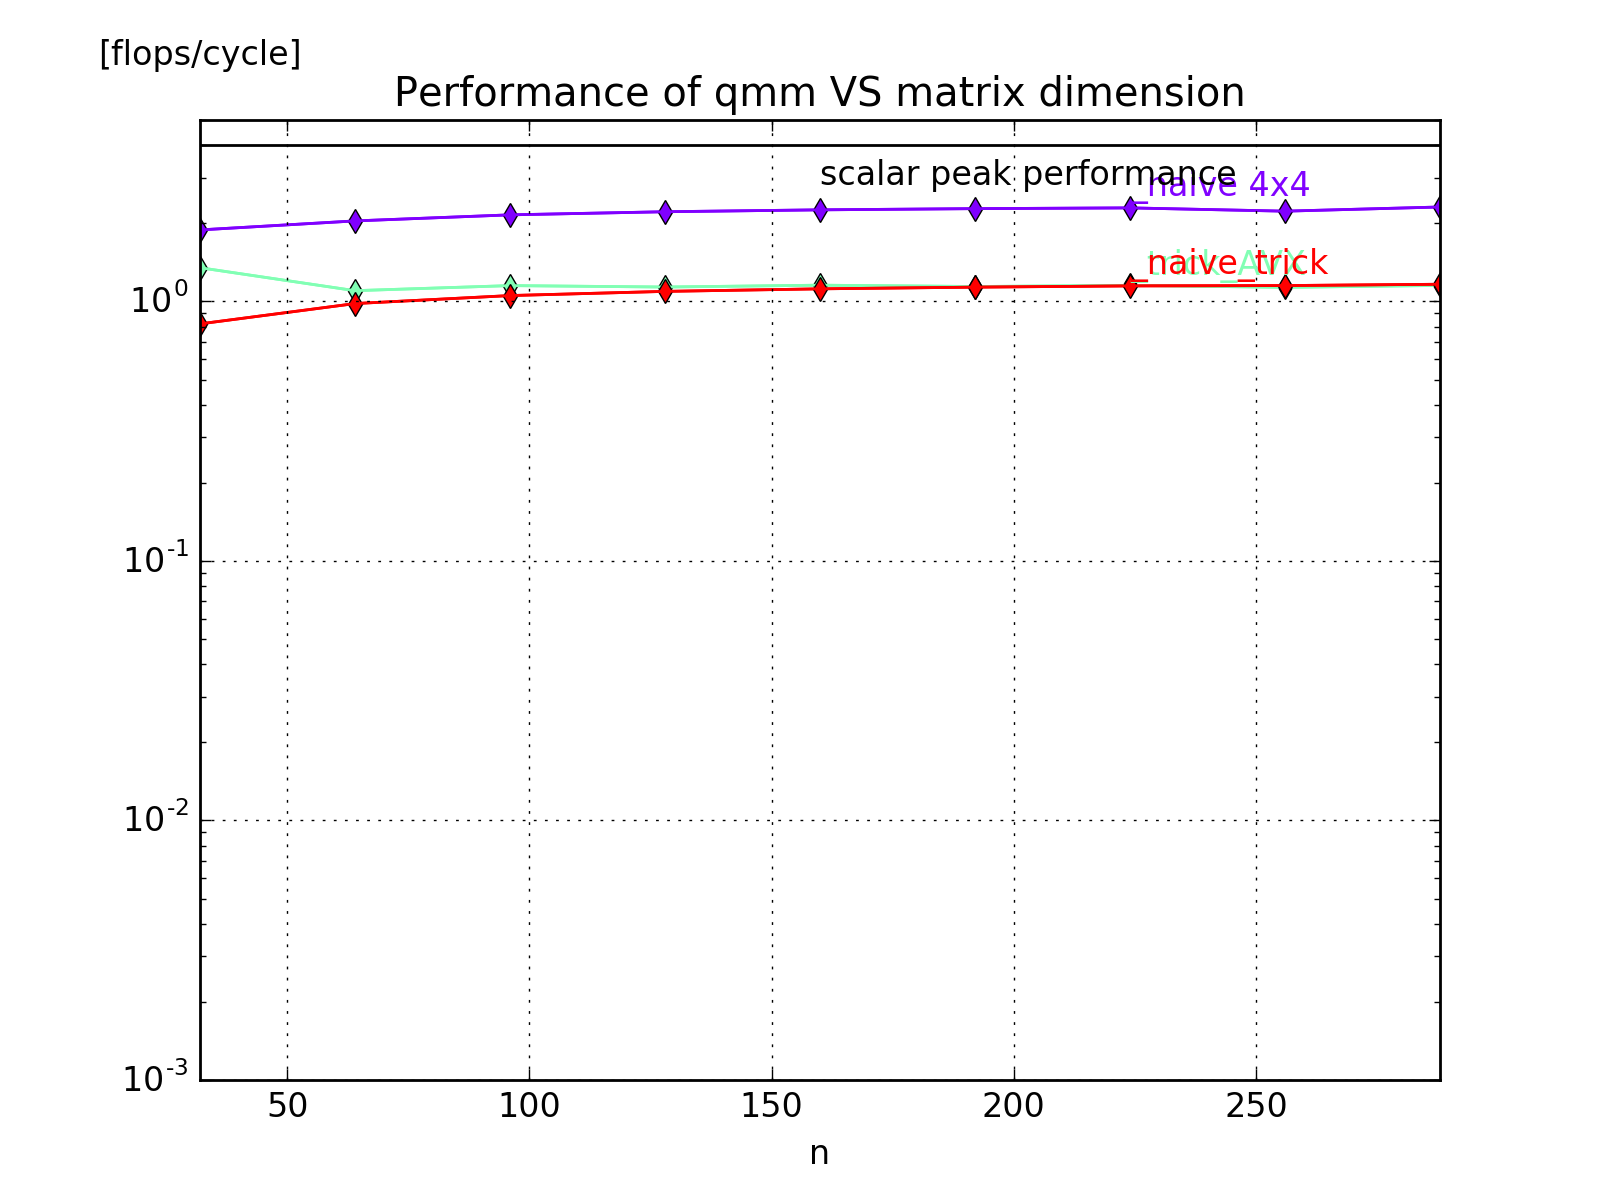
\includegraphics[width=0.5\textwidth]{Performance_qmm.eps}
\caption{Performance plot for the QMM kernel}
\label{figure:performance_qmm_kernel}

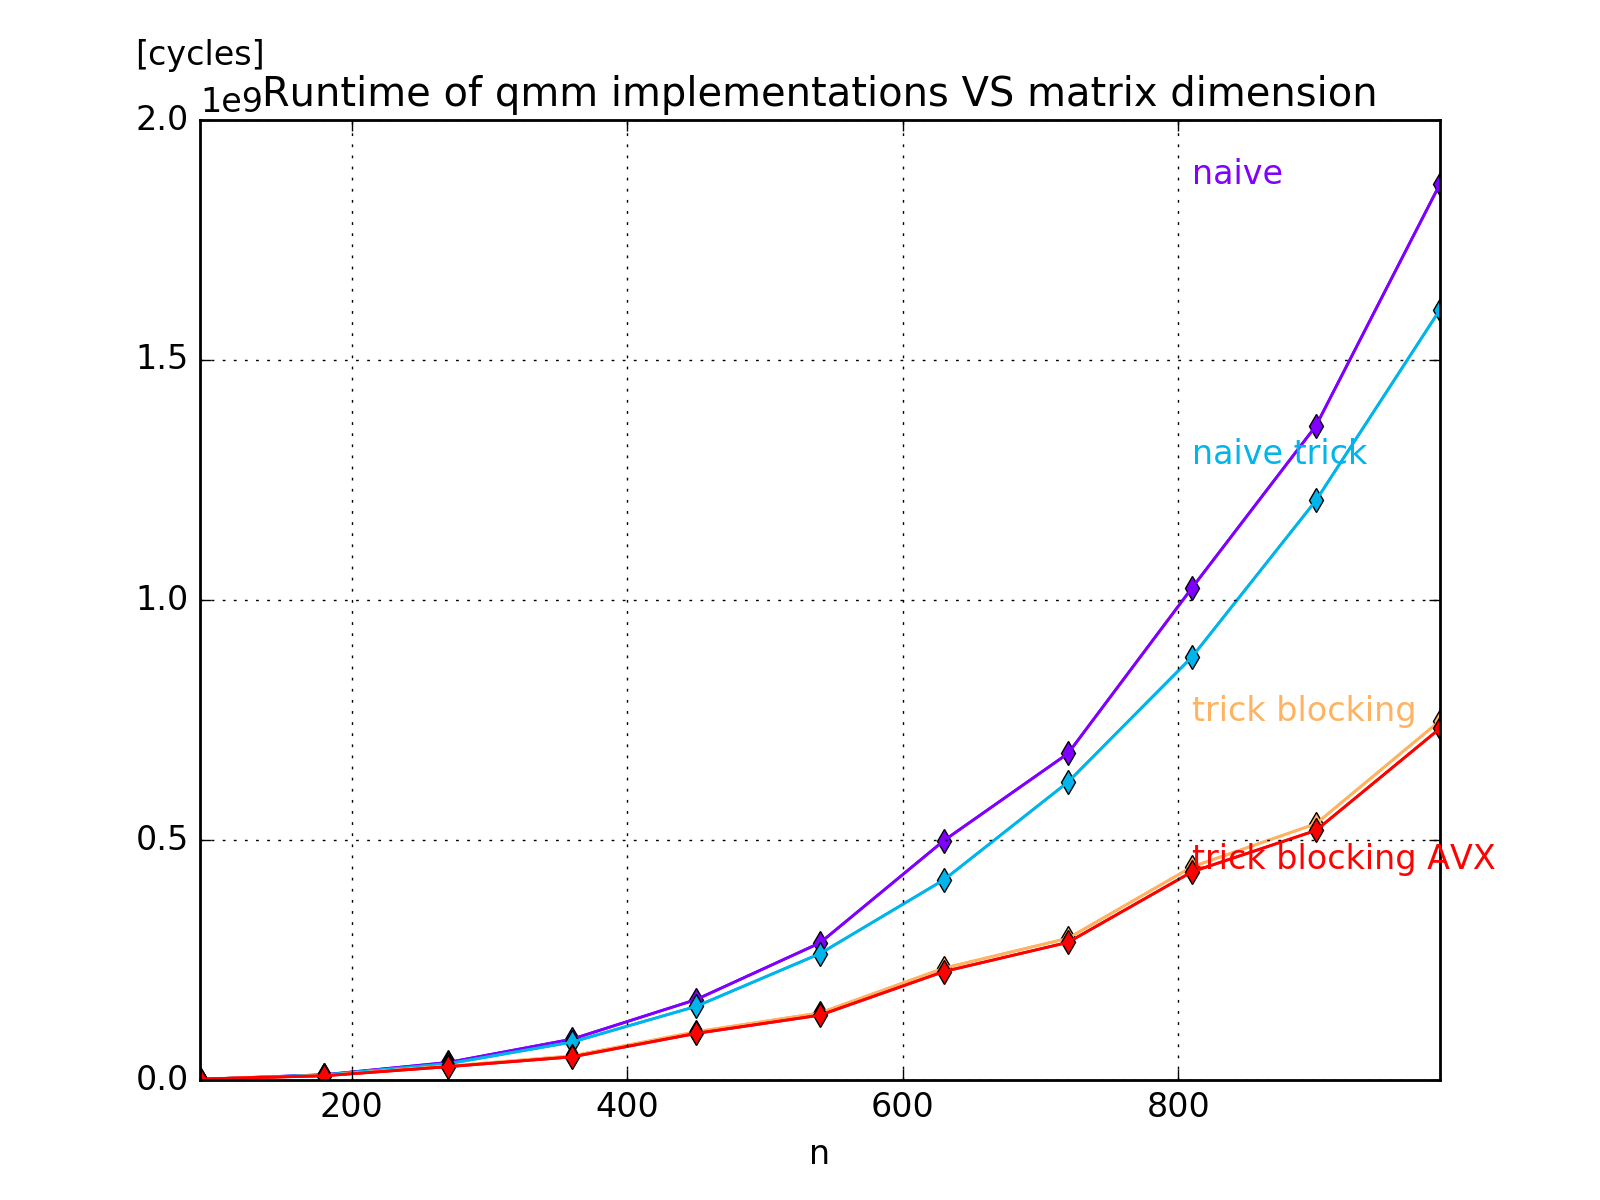
\includegraphics[width=0.5\textwidth]{Cycles_qmm_comparison.eps}
\caption{Runtime plot of the overall pipeline}
\label{figure:cycles_qmm_comparison}
\end{figure}

\begin{figure}[h]
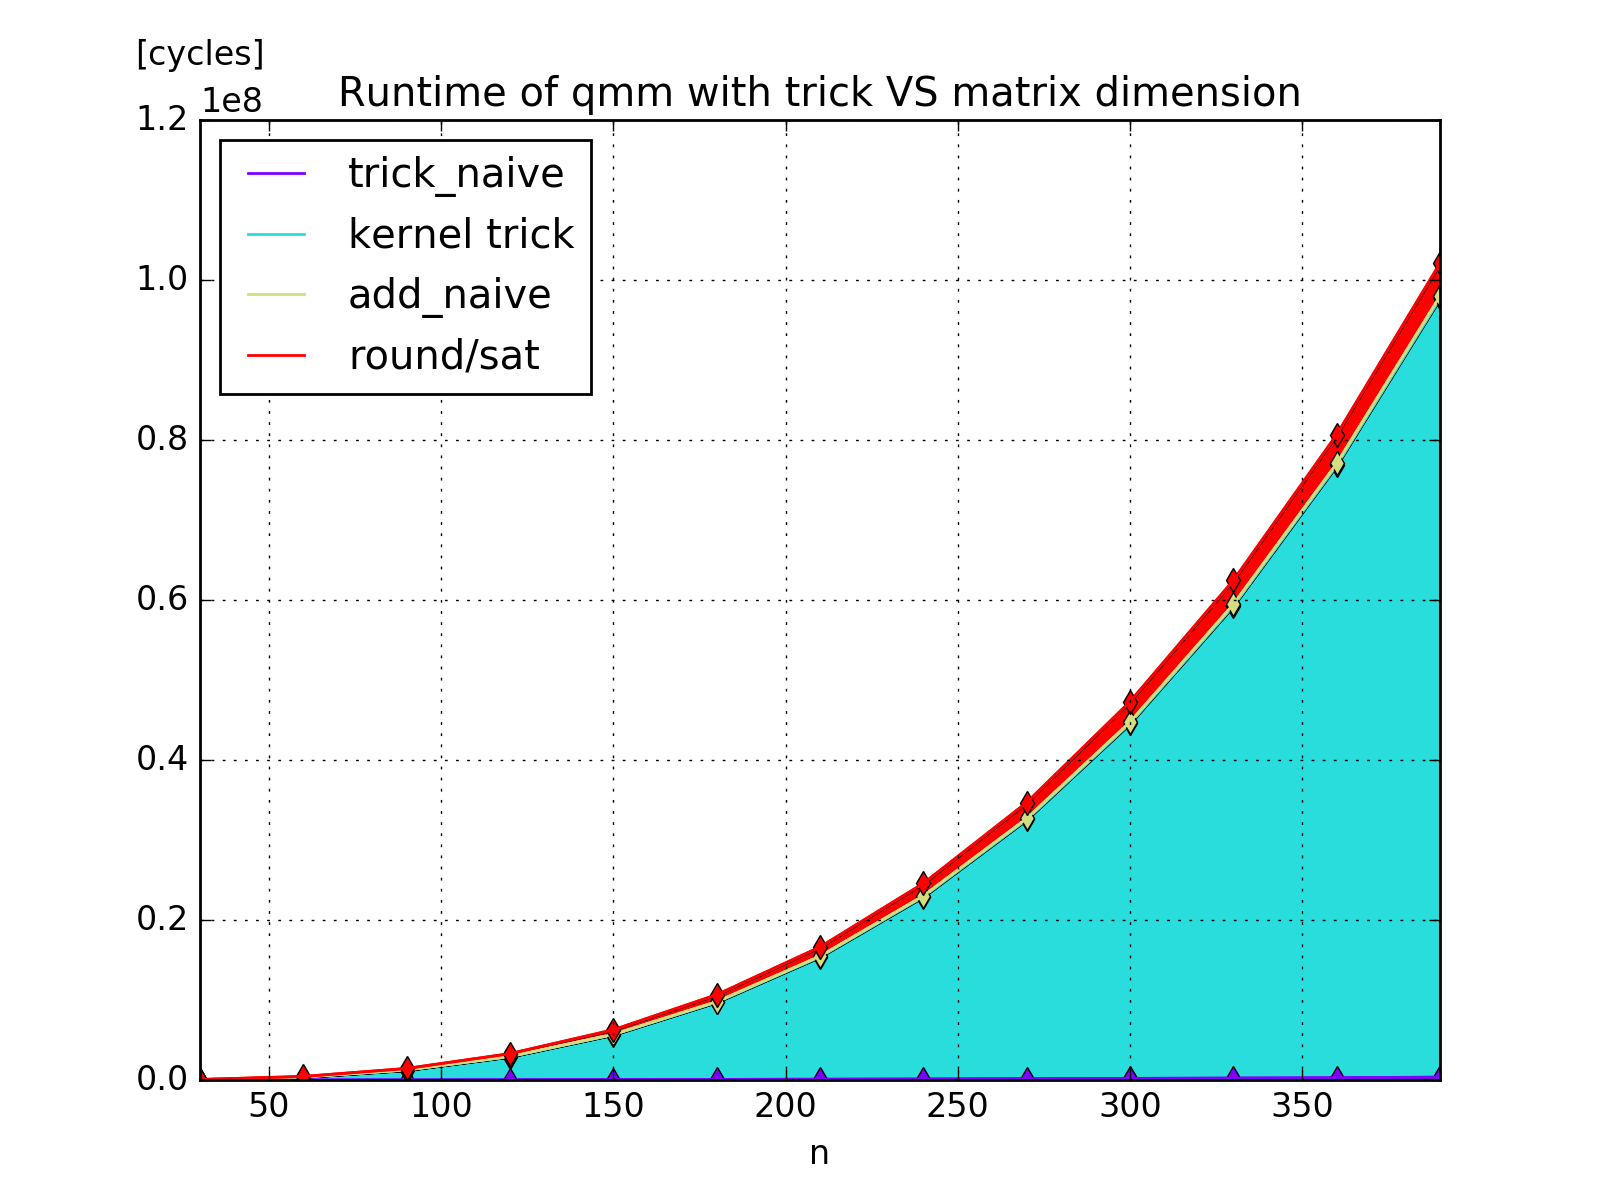
\includegraphics[width=0.5\textwidth]{Cycles_trick.eps}
\caption{Contribution of each naive-version sub-function in the overall runtime.} 
\label{figure:Cycles_trick}
\end{figure}


\mypar{Results: blocking for MMM}
The blocking parameter used is $N_b = 30$ for the cache blocking parameter and $n_b = 3$ for the register blocking parameter, as described in \cref{sec:yourmethod}. \cref{figure:performance_qmm_kernel} shows the gain in performance with respect to the naive\_trick implementation. The large $n$ performance gain is approximately $2$X. Note that the blocking parameter for cache and for register are not fine tuned, so a further speedup could be possible.

\begin{comment}
Next divide the experiments into classes, one paragraph for each. In the simplest case you have one plot that has the size on the x-axis and the performance on the y-axis. The plot will contain several lines, one for each relevant code version. Discuss the plot and extract the overall performance gain from baseline to best code. Also state the percentage of peak performance for the best code. Note that the peak may change depending on the situation. For example, if you only do additions it would be 12 Gflop/s
on one core with 3 Ghz and SSE and single precision floating point.

Do not put two performance lines into the same plot if the operations count changed significantly (that's apples and oranges). In that case first perform the optimizations that reduce op count and report the runtime gain in a plot. Then continue to optimize the best version and show performance plots.

{\bf You should}
\begin{itemize}
\item Follow the guide to benchmarking presented in class, in particular
\item very readable, attractive plots (do 1 column, not 2 column plots
for this class), proper readable font size. An example is below (of course you can have a different style),
\item every plot answers a question, which you pose and extract the
answer from the plot in its discussion
\end{itemize}
Every plot should be discussed (what does it show, which statements do
you extract).
\end{comment}

\mypar{Results: vectorization} 
In this paragraph we evaluate the performance gain of the vectorization of the sub-functions \emph{trick\_vector}, \emph{quantize}, \emph{add\_trick\_vector} and \emph{round\_saturation} as outlined in \cref{sec:yourmethod}. \cref{figure:performance_add_vector} and \cref{figure:performance_trick_vector} show a linear increase of the performance for small instances. This is due to a border effect. The instance size in the  performance plot are not in general a multiple of the vector size ($16$X$16 \ Bits$), hence for small instance size the scalar computation can be non-negligible. Moreover the scalar contribution decreases linearly with the size of the instance.

\begin{figure}[h]
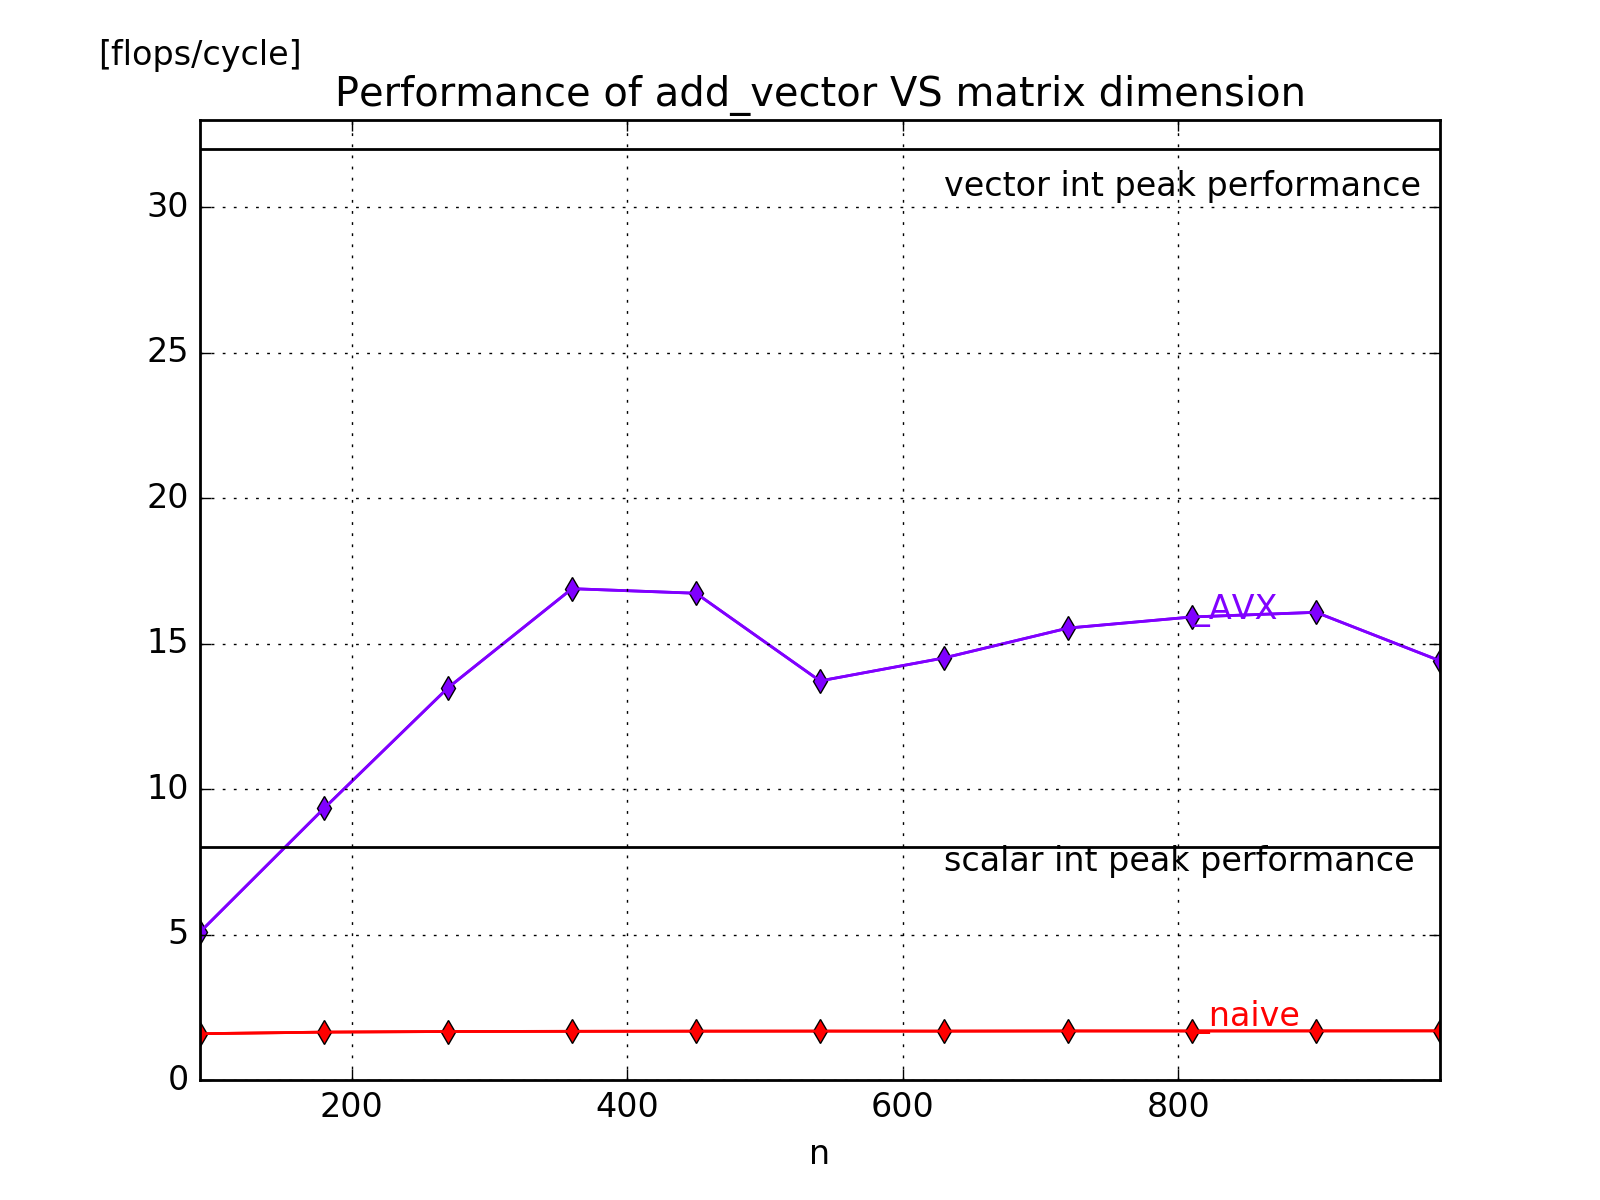
\includegraphics[width=0.5\textwidth]{Performance_add_vector.eps}
\caption{Performance plot of the function \emph{add\_vector}}
\label{figure:performance_add_vector}
\end{figure}

\begin{figure}
	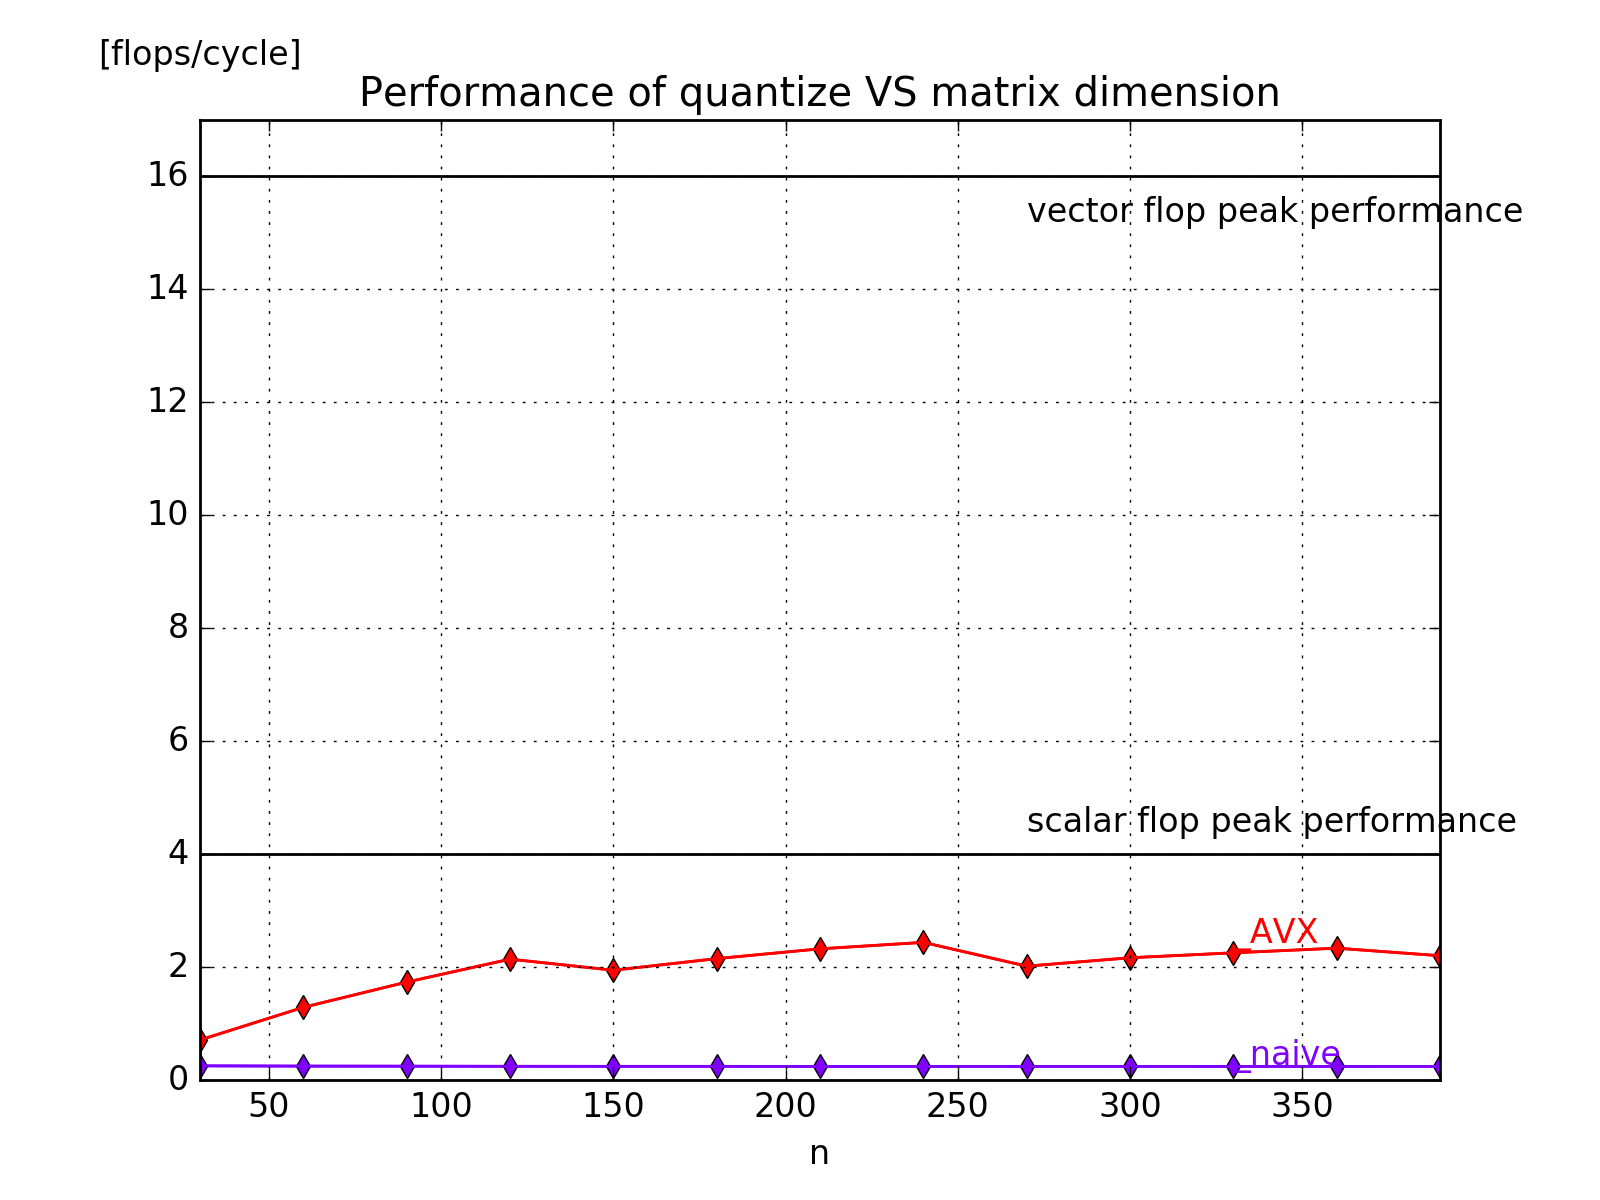
\includegraphics[width=0.5\textwidth]{Performance_quantize.eps}
	\caption{Performance plot of the function \emph{quantize}}
	\label{figure:performance_quantize}
\end{figure}

\begin{figure}
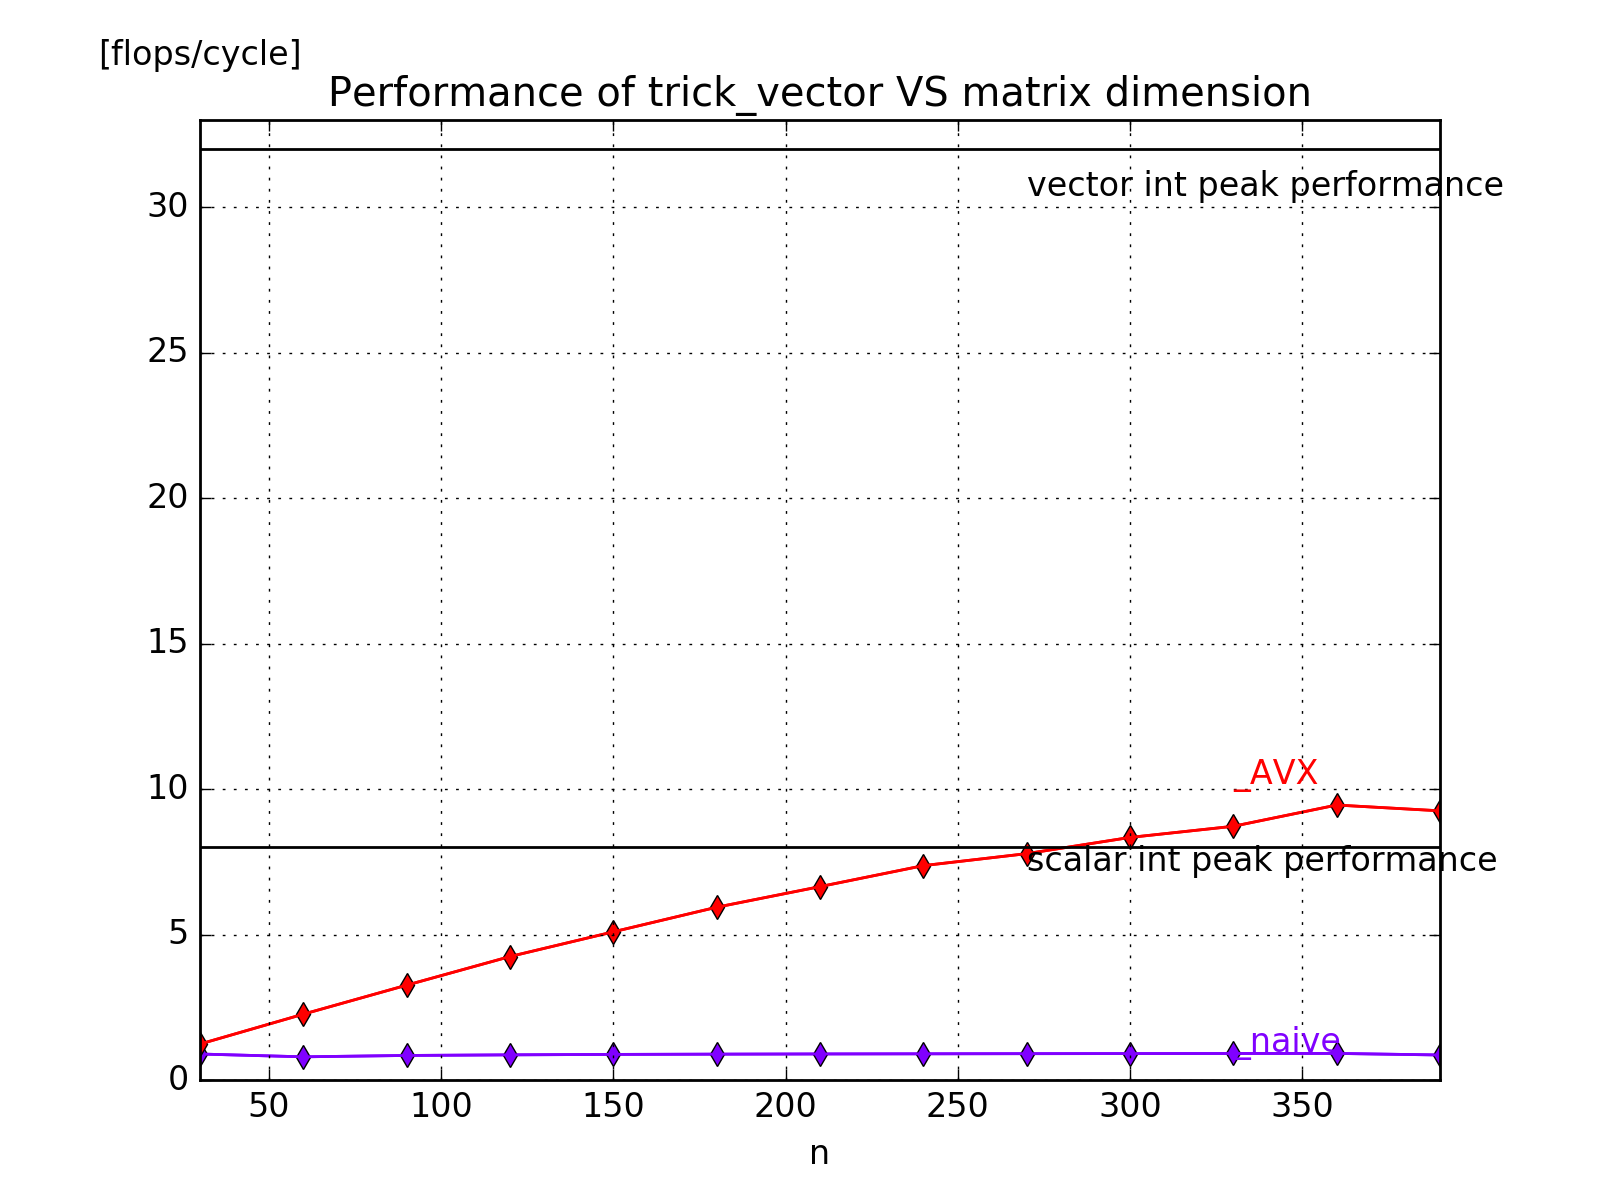
\includegraphics[width=0.5\textwidth]{Performance_trick_vector.eps}
\caption{Performance plot of the function \emph{trick\_vector}}
\label{figure:performance_trick_vector}
\end{figure}

\begin{figure}
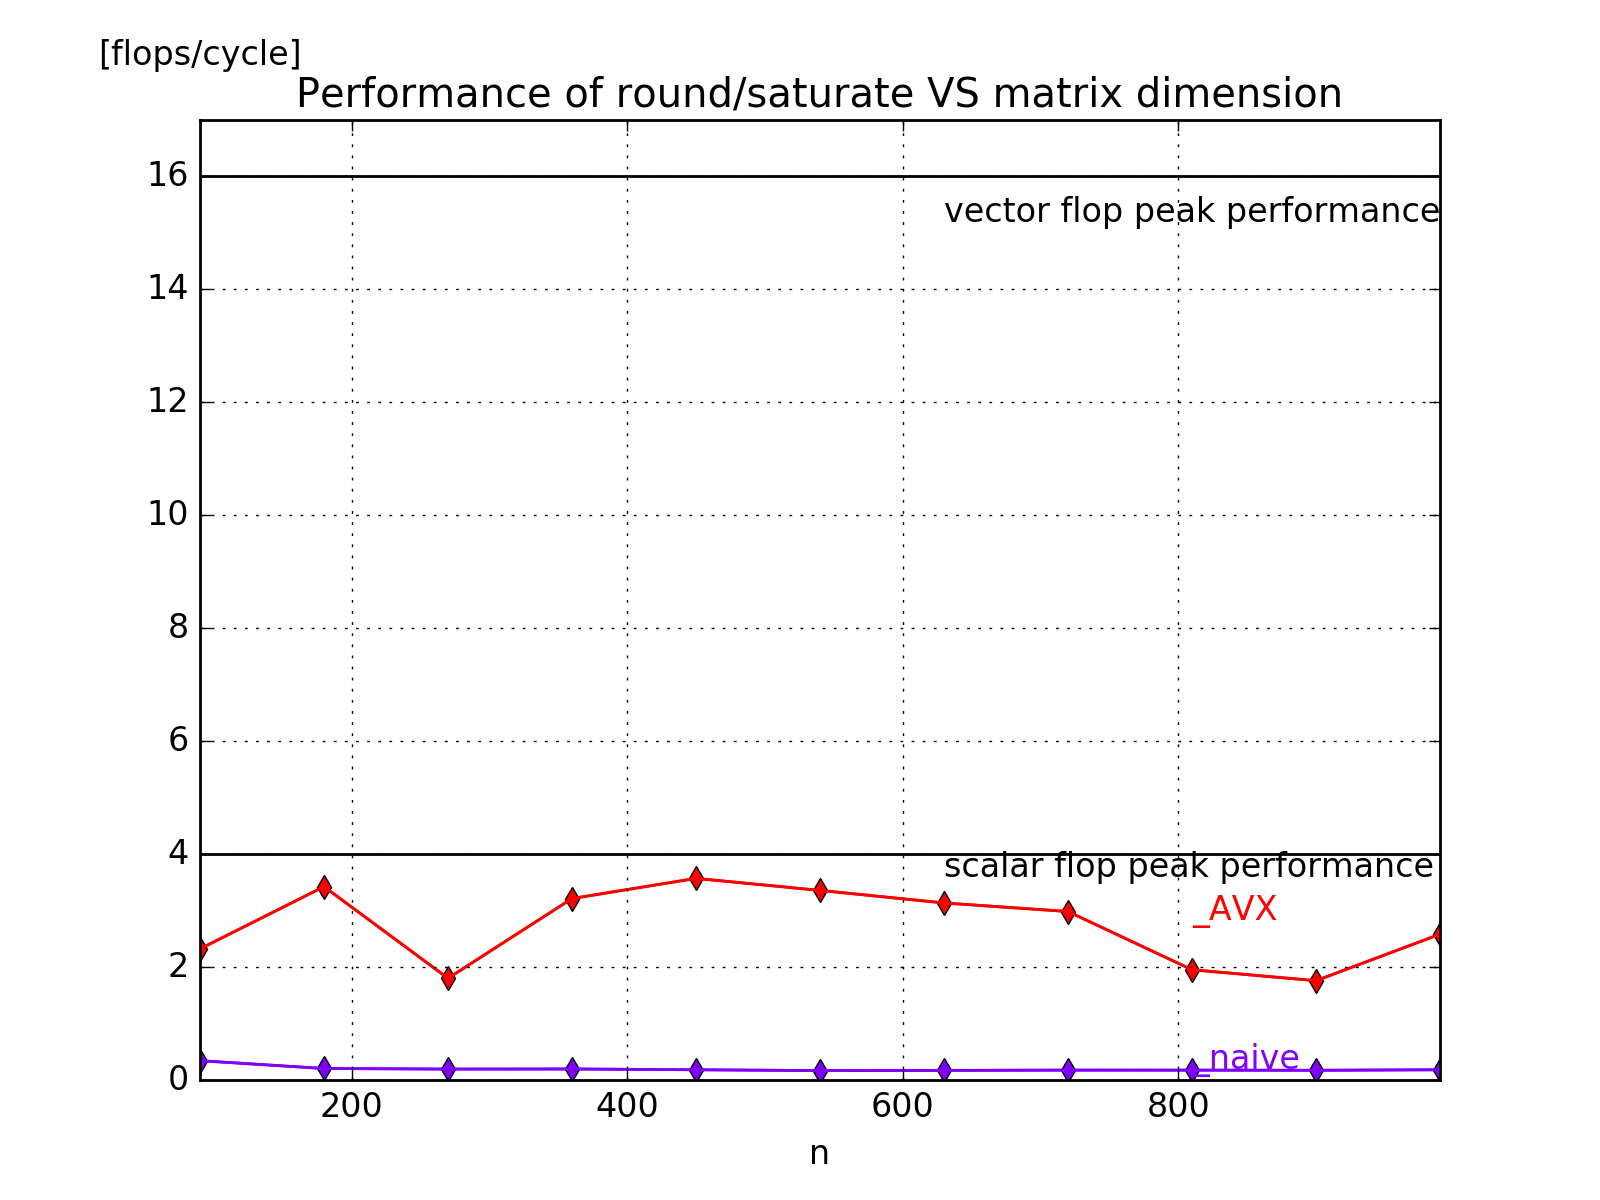
\includegraphics[width=0.5\textwidth]{Performance_round_saturation.eps}
\caption{Performance plot of the function \emph{round\_saturation}}
\label{figure:performance_round_saturation}
\end{figure}

The maximal gain in performance that the vectorization can allow for the integer functions \emph{trick\_vector} and \emph{add\_trick\_vector} is $16$X, that is the size of the accumulator vector. The measured performance gain are respectively  $9.8$X and $8.5$X.

\cref{figure:performance_quantize} and \cref{figure:performance_round_saturation} show the performance plot for the functions \emph{quantize} and \emph{round\_saturation}. The measured performance gain are respectively $9.2$X and $14.2$X. 

In \cref{figure:cycles_qmm_comparison} we can see the runtime plot for the whole pipeline. The implementation \emph{trick\_blocking\_AVX} is obtained combining the \emph{QMM\_kernel\_blocking} with the vectorized implementation of all the other sub-functions. The overall speedup is $2.5$X.